\begin{figure*}
  %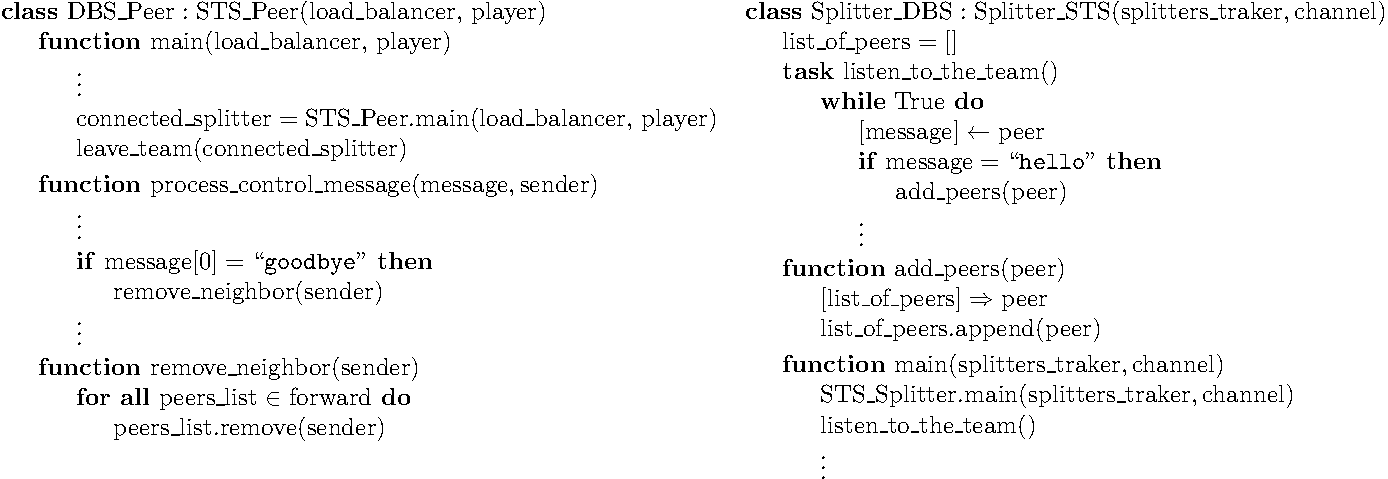
\includegraphics[width=0.55\textwidth]{leaving}
  \fig{300}{4cm}{leaving}
  \caption{Peer leaving.\label{fig:leaving}}
\end{figure*}
An outgoing peer $P^j_o$ (see Fig.~\ref{fig:leaving}) must to: (1) say
$[\mathtt{goodbye}]$ to $S^j$ and to $T^j_o$ (in this order), (2)
relay any pending (received but yet not sent) chunks, and (3) wait for
a $[\mathtt{goodbye}]$ from $S^j$, which performs $T^j = T^j \setminus
P^j_o$. In case of a timeout, $P^j_o$ resets the leaving procedure,
for a maximum number of times.

When a $P^j_k$ receives a $[\mathtt{goodbye}]$ from $P^j_o$, $P^j_k$
removes $P^j_o$ from its neighbors set, by running $T^j_k = T^k_j
\setminus P^j_o$.
